%%%%%%%%%%%%%%%%%%%%%%%%%%%%%%%%%%%%%%%%%%%%%%%%%%%%%%%%%%%%%%%%%%%%%%%%%%%%%%%%
%2345678901234567890123456789012345678901234567890123456789012345678901234567890
%        1         2         3         4         5         6         7         8

% \documentclass[letterpaper, 10 pt, conference]{ieeeconf}  % Comment this line out if you need a4paper

\documentclass[a4paper, 11.5pt, conference]{ieeeconf}      % Use this line for a4 paper

\IEEEoverridecommandlockouts                              % This command is only needed if 
                                                          % you want to use the \thanks command

\overrideIEEEmargins                                      % Needed to meet printer requirements.

%In case you encounter the following error:
%Error 1010 The PDF file may be corrupt (unable to open PDF file) OR
%Error 1000 An error occurred while parsing a contents stream. Unable to analyze the PDF file.
%This is a known problem with pdfLaTeX conversion filter. The file cannot be opened with acrobat reader
%Please use one of the alternatives below to circumvent this error by uncommenting one or the other
%\pdfobjcompresslevel=0
%\pdfminorversion=4

% See the \addtolength command later in the file to balance the column lengths
% on the last page of the document

% The following packages can be found on http:\\www.ctan.org
\usepackage{graphics}
%\usepackage{parskip} % for pdf, bitmapped graphics files
%\usepackage{epsfig} % for postscript graphics files
\usepackage{mathptmx} % assumes new font selection scheme installed
\usepackage{times} % assumes new font selection scheme installed
\usepackage{amsmath} % assumes amsmath package installed
\usepackage{amssymb}  % assumes amsmath package installed
\usepackage{float}
\usepackage{subcaption}
\usepackage{caption}
\usepackage{hyperref}
\hypersetup{hidelinks}
\title{\LARGE \bf Collision Monitoring for a Mobile Manipulator Based on Biologically-Inspired Dynamical Systems for Movement Generation}
\usepackage[colorinlistoftodos]{todonotes}

\author{Sreenivasa Hikkal Venugopala, Zain Ul Haq, and Urvashi Negi \\ {\small \textbf{Advisor:} Djordje Vukcevic}}
\setlength{\parskip}{0pt}

\begin{document}



\maketitle
\thispagestyle{empty}
\pagestyle{empty}


%%%%%%%%%%%%%%%%%%%%%%%%%%%%%%%%%%%%%%%%%%%%%%%%%%%%%%%%%%%%%%%%%%%%%%%%%%%%%%%%
\begin{abstract}
The computations involving the robotic manipulators, that is robotic arms and the mobile manipulators, that is mobile base (robot base) up until recent times are limited in the degree of operation and have several restrictions due to rigid movements, the control algorithms for these manipulators are usually complex involving various operations such as planning, perception, and so on. This makes the computations complex and time consuming and make it hard for its usage in the dynamic environments involving other robots, humans. To overcome these issues, in this research work, we propose to extend the implementation of the control algorithms which is implemented based on collision monitoring \cite{Khatib} and collision avoidance \cite{Hoffmann} for controlling the movements of the robotic arms from colliding each other and to extend it to avoid collision with the mobile base as well. Along with this, we also implement the control algorithms for mobile base that helps in monitoring and avoiding the collision with any obstacles and helps in safe maneuvering towards the goal.

\end{abstract}


%%%%%%%%%%%%%%%%%%%%%%%%%%%%%%%%%%%%%%%%%%%%%%%%%%%%%%%%%%%%%%%%%%%%%%%%%%%%%%%%
\section{Introduction} 

%Background ---------------
The robotic arms or the robotic manipulators are used in various applications ranging from industrial applications to domestic applications. They are widely used in industrial applications such as to support human in the production lines of heavy machineries for the purpose of assembling spare parts, welding, painting and so on, and in domestic applications such as robotic prosthetics, robotic assistants, and so on. Along with these applications, A robot as a whole, that is including both arms and the mobile base, poses useful in various applications such as warehouse management. All these applications require more robust and highly adaptable software and hardware components. For increasing the efficiency and the robustness of the functioning of the robotic manipulators in industrial applications, a precomputed trajectories will be provided \cite{Hoffmann}, but these precomputed trajectories will not consider the dynamic movement of human and other obstacles. On the other hand, various operators are used to control the movement and functioning of the robotic prosthetics, but this does not provide free flow motion for the arms or prosthetics. On contrary it takes a lot of time and effort to train the robotic manipulators to perform a safe and free flow movement, but this is a high cost solution which is not weighable in all scenarios.

One of the solution approach to handle the control algorithm problem is to make use of the dynamic movement primitives, these are generated during the movement of the robot manipulators resulting in real-time collision monitoring and avoidance. There were many approaches proposed as a solution to this problem, based on the approaches proposed by \cite{Hoffmann} and \cite{Khatib} a library named `Implementation of biologically-inspired dynamical systems for
movement generation: automatic real-time goal adaptation and obstacle avoidance' was developed (\url{https://github.com/HBRS-SDP/sdp\_ss20\_collision\_monitoring\_for\_robotic\_manipulators}). This library handles the collision monitoring and collision avoidance for robotic arms in real-time and it incorporates the idea of dynamic movement primitives and the potential field method for active collision monitoring and avoidance. Here the dynamic primitives and the obstacles are considered as the basic primitives having shape and volume.

In this work, we propose to implement and extend the previous work by formulating the mobile manipulator or the robot base as a 3D box shape and extend the control algorithm to avoid and monitor the collision between the robot arms and its base. Along with this we also implement the control algorithm for the base to avoid and monitor the base from colliding with other obstacles. Initially we planned and tried to model the base as a convex hull using the approach proposed by \cite{GJK}, and it turned out to be complex and cost ineffective for this application. To overcome this, we modeled the robot base to be a 3D box and calculate the distance between other dynamic primitives which are discussed in the future sections. Extension of previous work to monitor and avoid collision between the arms and the base, along with implementation of the control algorithm for controlling the base from avoiding and active monitoring of collision makes the robot more robust, adaptable, and safe to use in dynamic environments including for domestic purposes.

This report is further structured as follows. Section 2 describes modeling and  calculating the distances between the dynamic primitives, Section 3 highlights the implementation details, Section 4 describes various experiments conducted, and Section 5 provides information on use cases followed by the conclusion.
%Robotic assistants

\section{Approach}

\subsection{Distance between primitives}
In previous work, the links and joints, along with the end-effector and obstacles were modeled as spheres and cylinders. In this work, along with the previous implementations, we model the robot base as a 3D box, this helps in easier calculations for the distance between the arms and robot body, and robot body and other obstacles. Following we will discuss the distance calculations between various primitive objects.

1) Distance between two spheres:
We calculate distance between two spheres using below formula:
\begin{equation}
	Distance = |\bar{C_1}-\bar{C_2}| - (r_1 + r_2)
\end{equation}
where $\bar{C_1}$ and $\bar{C_2}$ represent the center points of the two spheres, and $r_1$ and $r_2$ are the radius the two spheres and the same is visualized in Figure \ref{fig:sphere_sphere}.

\begin{figure}[H]
    \centering
    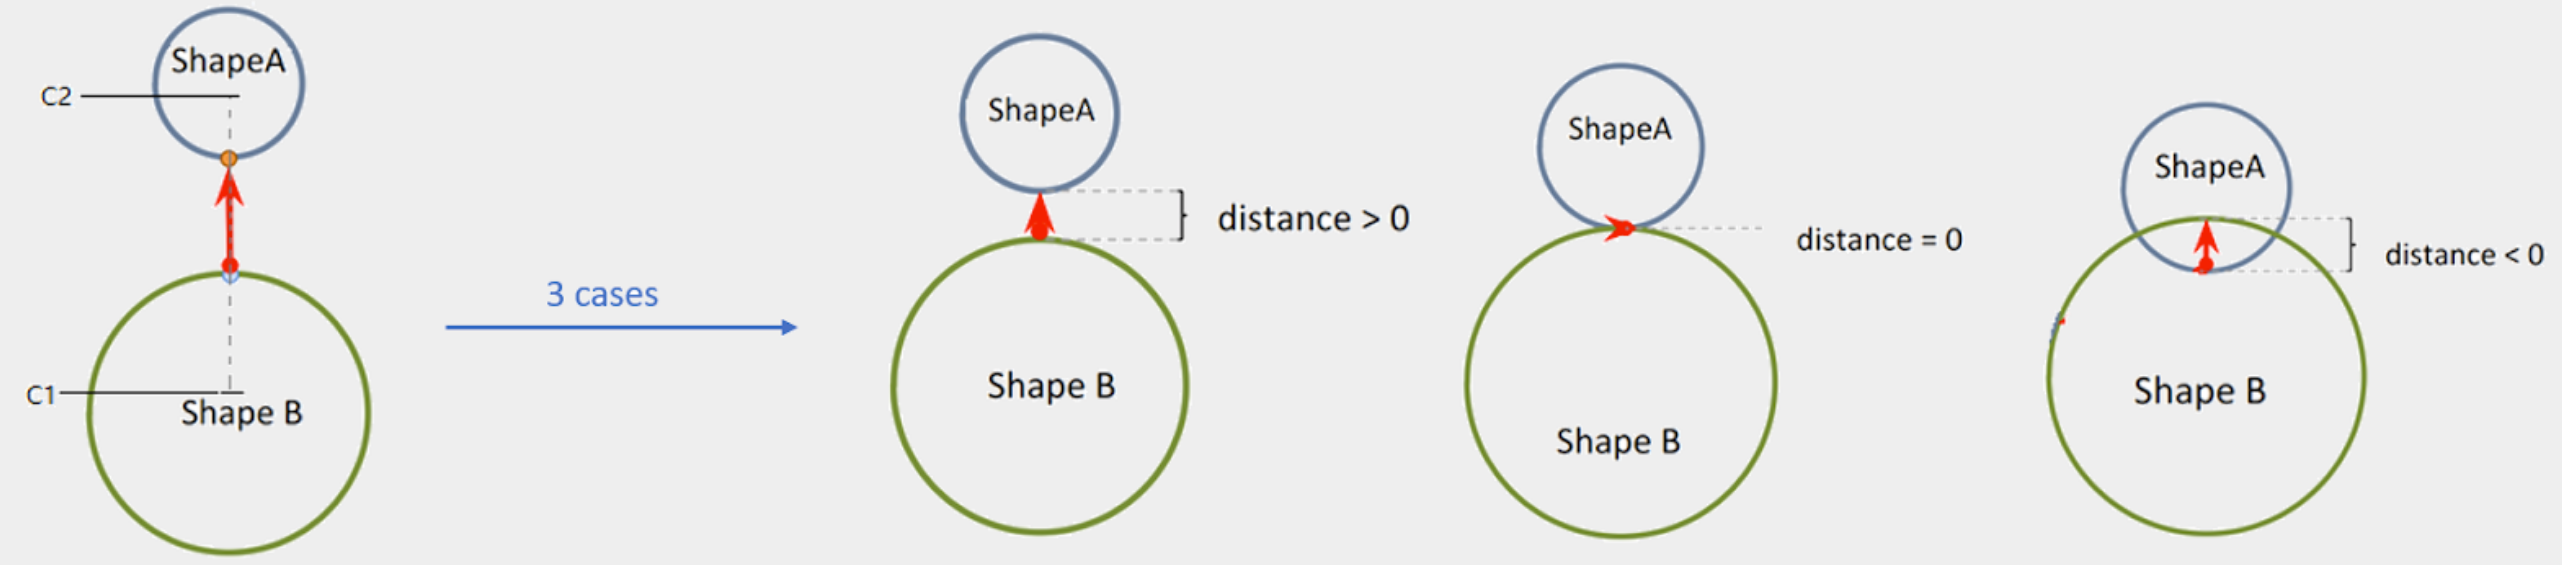
\includegraphics[scale=0.23]{images/sphere_sphere.png}
    \caption{Sphere - sphere}
    \label{fig:sphere_sphere}
\end{figure}

2) Distance between sphere and cylinder:
We calculate the distance between the sphere and a cylinder using below equation and the same is shown in the Figure \ref{fig:spherecapsule}.
\begin{equation}
	Closest point = X = 	\begin{cases}
        x = x_1 + \lambda(x_2 - x_1) \\
        y = y_1 + \lambda(y_2 - y_1) \\
        z = z_1 + \lambda(z_2 - z_1) 
    \end{cases}
    \label{eq:cpcyl}
\end{equation}

\begin{equation}
	\lambda = \frac{(c-m_1).(m_2-m_1)}{La^2}
\end{equation}

\begin{equation}
	Distance = |X-C| - (r_a + r_s)
\end{equation}

\begin{figure}[H]
    \centering
    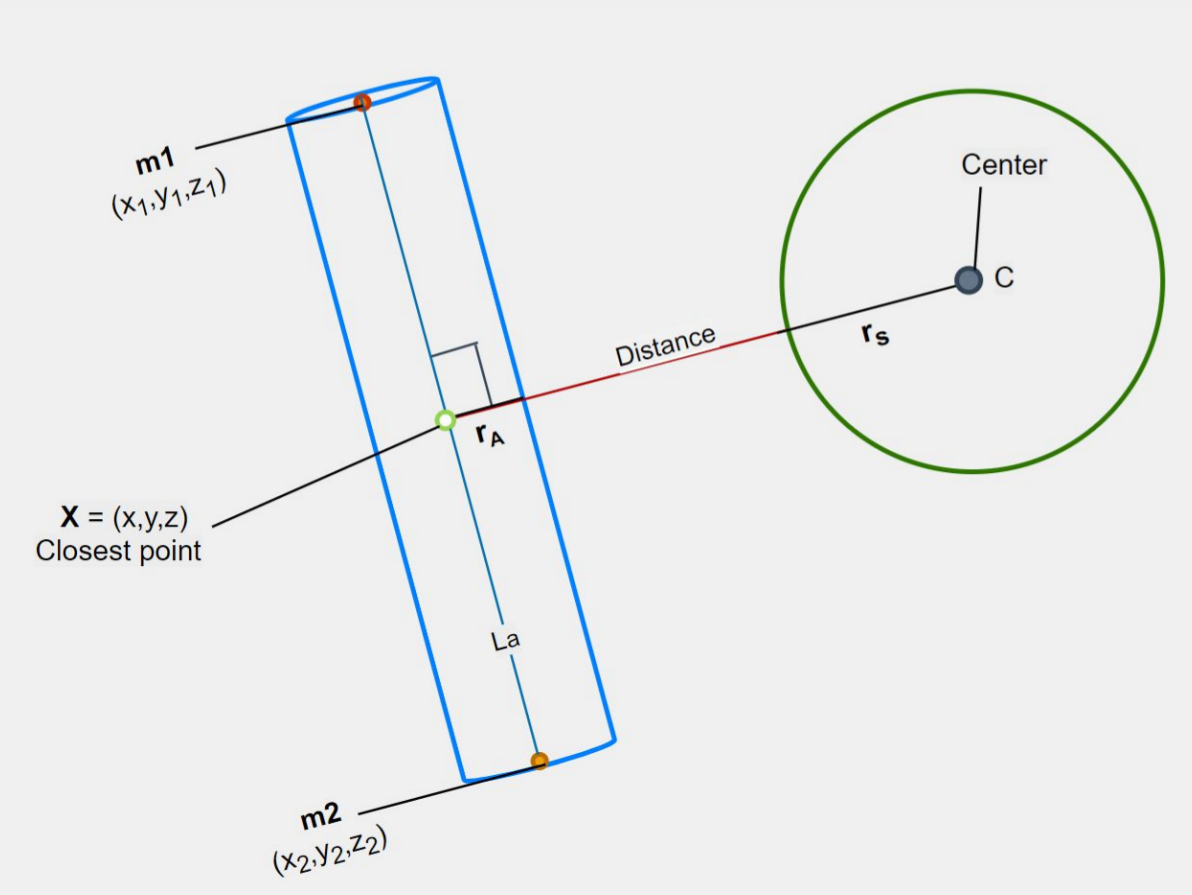
\includegraphics[scale=0.3]{images/sphere_capsule.png}
    \caption{Sphere - capsule}
    \label{fig:spherecapsule}
\end{figure}

3) Distance between two cylinders:
We compute the distance between the two cylinders based on the following four cases:
\begin{enumerate}
	\item m1 and m2 can be perpendicularly projected on to La.
	\item m1 and m2 cannot be perpendicularly projected on to La.
	\item Only m2 can be perpendicularly projected on to La.
	\item Only m1 can be perpendicularly projected on to La.
\end{enumerate}
Here, m1 and m2 refers to the starting point and end point of the symmetrical axis of shorter cylinder, La is the symmetrical axis of the longer cylinder. This is shown in Figure \ref{fig:capsule_capsule}.
\begin{figure}[H]
    \centering
    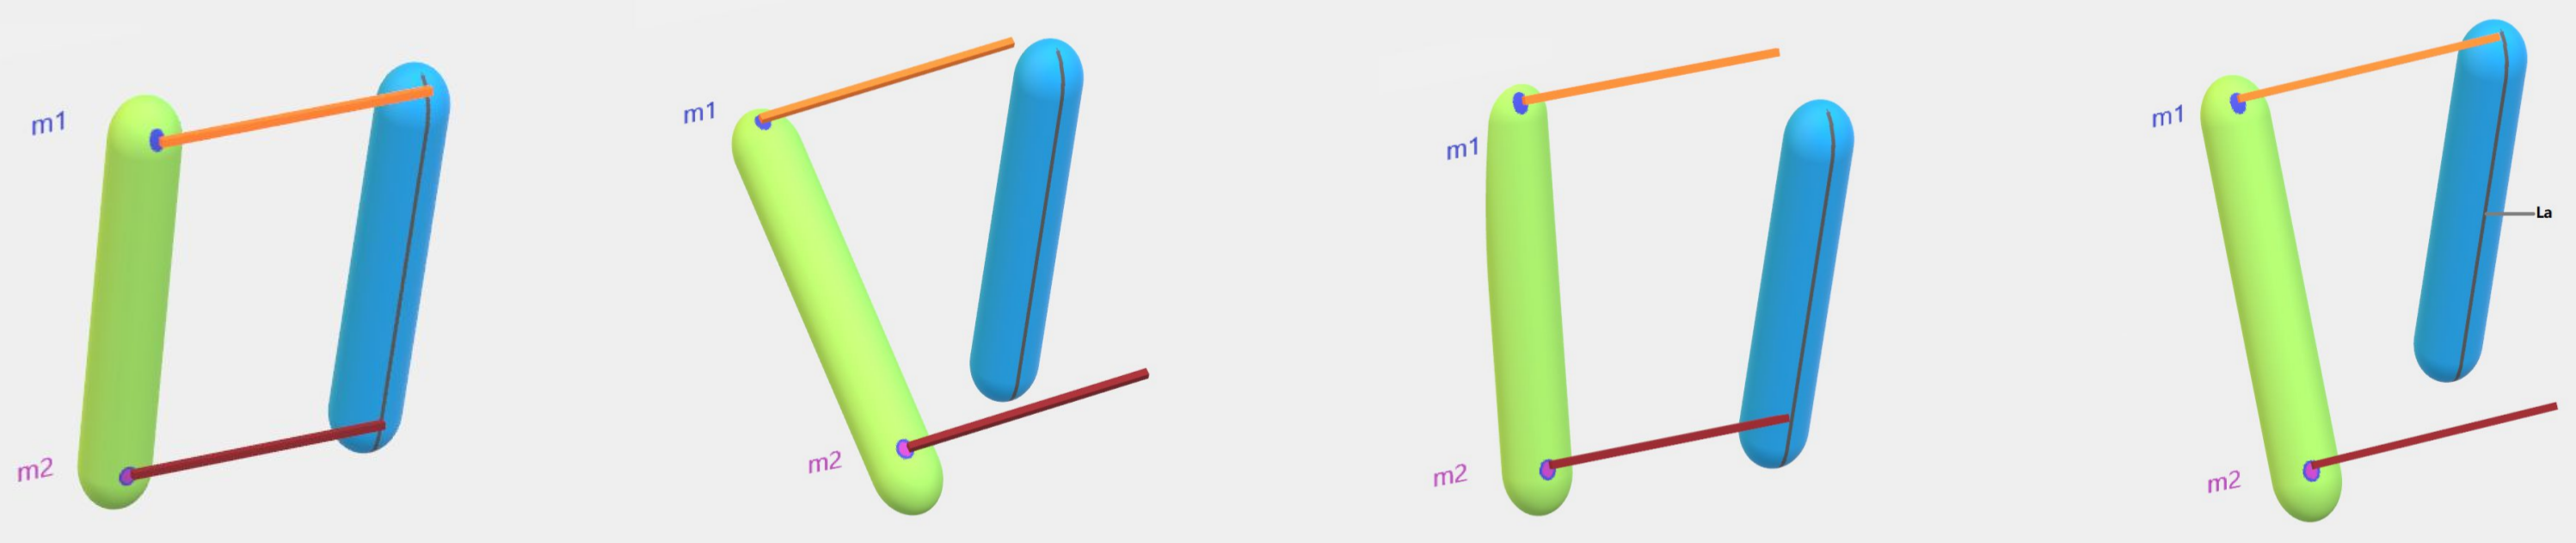
\includegraphics[scale=0.21]{images/capsule_capsule.png}
    \caption{Cylinder - cylinder}
    \label{fig:capsule_capsule}
\end{figure}

4) Box configuration and closest point on the box:
As an extension to previous work, here we have modeled the robot base as a 3D box or of cuboid shape. This box is considered as Axis Aligned Bounding Box (AABB) \cite{3ddet}, it means that the AABB doesn't have to have equal length, width, and height, but one condition here is that once it is configured the box should not be rotated. These AABBs are pivotal towards spatial partitioning. An example visualization is provided in Figure \ref{fig:aabb}. These boxes can be stored in two ways, first is to store the leftmost and rightmost corners and the second way is to store the center point of the box and a vector representing how far it extends in each x, y, z directions.

\begin{figure}[H]
    \centering
    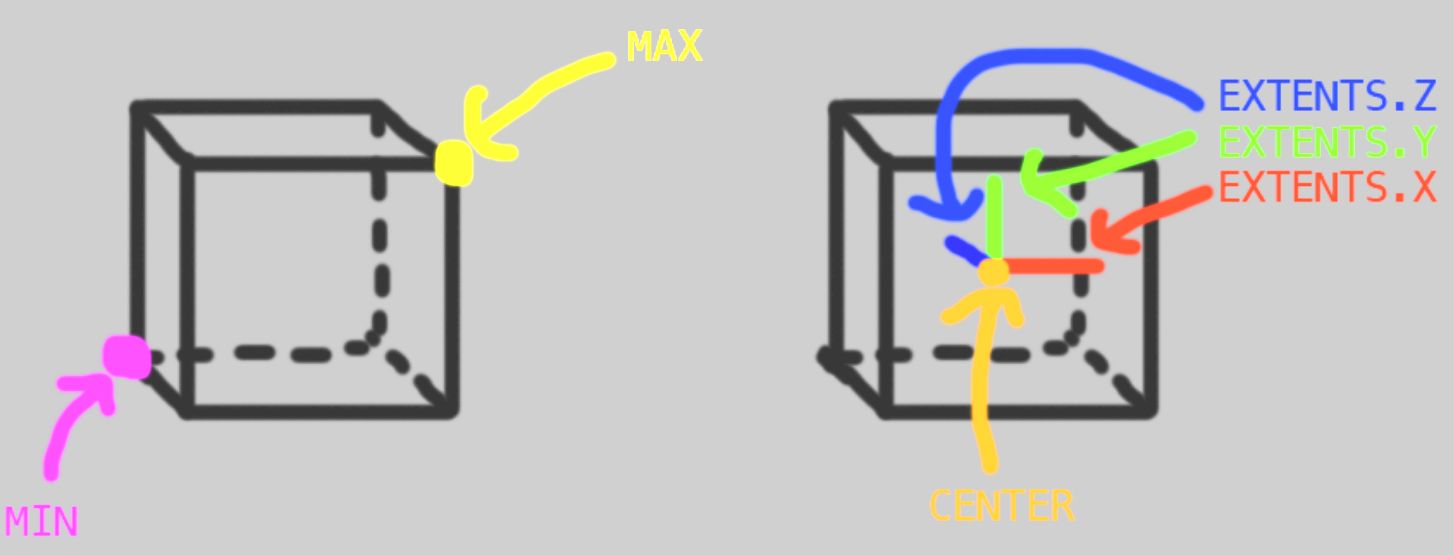
\includegraphics[scale=0.3]{images/aabb.png}
    \caption{Representation of AABB, image referenced from \cite{3ddet}}
    \label{fig:aabb}
\end{figure}

Initially we check if the given point is inside or on the box by comparing it to the position of leftmost corner (min) and rightmost corner (max). Since box has many edges and sides, we do have to figure out the closest point on the box that is closest to the obstacle. The algorithm to determine the closest point shows that the point will be clamped to AABB, that is we check if the point is outside the box and then compare the position of point with respect to min and max of the AABB and clamp the point to the nearest edge based on this comparison. If the point is inside the box, then the algorithm just returns the position of the point itself.

5) Distance between box and sphere:
To find the distance between the box and the sphere, first we have to consider the distance between the center of the sphere and the closest point on AABB. To find out the closest point of AABB we consider the sphere center to be the point of consideration. Once we have the closest point on box, we calculate the distance by using Equation \ref{eq:boxsp}. If this distance is less than the radius of the sphere, then we say that the box and sphere are intersecting \cite{3ddet}.

\begin{equation}
	Distance = Sphere.Position - ClosestPoint
	\label{eq:boxsp}
\end{equation}

6) Distance between box and cylinder:
To find the distance between the box and the cylinder, fist we have to determine the closest point on the cylinder or capsule using the Equation \ref{eq:cpcyl}. We then clamp this closest point on to the AABB to find the closest point on the box. Once we have the two closest points, we consider the closest point of the cylinder or capsule to be the center point of the sphere and continue with the calculations by using the Equation \ref{eq:boxsp}. If this distance is less than the radius of the sphere (that is considered from the closest point on the cylinder or capsule to the edge of cylinder or capsule), then we say that the box is colliding with the cylinder or sphere \cite{3ddet}.

\subsection{Potential field calculations}
In previous work, to avoid and monitor the collision between the robotic arms and the obstacles, the algorithm from \cite{Hoffmann} is implemented. This algorithm is based on the dynamic movement primitives (DMP) and is used to generate the new trajectories and velocities in real-time as given in below equations,
\begin{equation} \label{eq:1}
	\dot{v} = K ( g - x ) - D v - K (g - x_0) s + K f(s) + p(x, v)
\end{equation}
Where $g$ is goal position, $x$ is current position, $x_0$ is starting position, $v$ is current velocity, $s$ is phase variable, $D$ is damping constant, and $K$ is spring constant. The term $p(x,v)$ refers to the potential field generated by the obstacles which in turn helps in avoiding obstacles.

This potential field is calculated by determining the steering angle (Figure \ref{steering_image}) between the velocity vector and the vector from the obstacle to the end effector as shown in \ref{eq:2}. This steering angle provides information on the sharpness of the steering of end effector from obstacle. Using this angle, the potential field is calculated as given in Equation \ref{eq:3}.

\begin{figure}[H]
	\centering
	\scalebox{0.55}{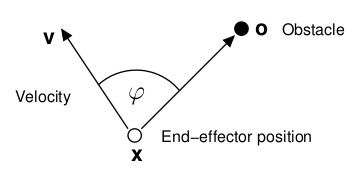
\includegraphics{images/steering_angle.png}}
	\caption{Graphical representation of steering angle \cite{Hoffmann}}
	\label{steering_image}
\end{figure}

\begin{equation} \label{eq:2}
	\varphi = cos^{-1}\Bigg( \frac{(o-v)^T v}{\|o-x\| \cdot \|v\|}\Bigg)
\end{equation}
\begin{equation} \label{eq:3}
	p(x, v) = \gamma \sum_i R_i v \varphi_i exp(-\beta \varphi_i) 
\end{equation}

Where $\gamma$ and $\beta$ are tune-able constants, and R is a rotation matrix which rotates by the axis $r = (o-x) \times v $ with an angle of rotation of $\pi/2$. This rotation matrix can be calculated using the following approach described in \cite{rodrigues}. The final potential field is the sum of the potential fields generated by all the obstacles. The final equation converges towards the goal avoiding the obstacles as given below.

\begin{equation}
\dot{v} = K ( g - x ) - D v + p(x, v)
\end{equation}

\begin{figure*}[t]
	\centering
	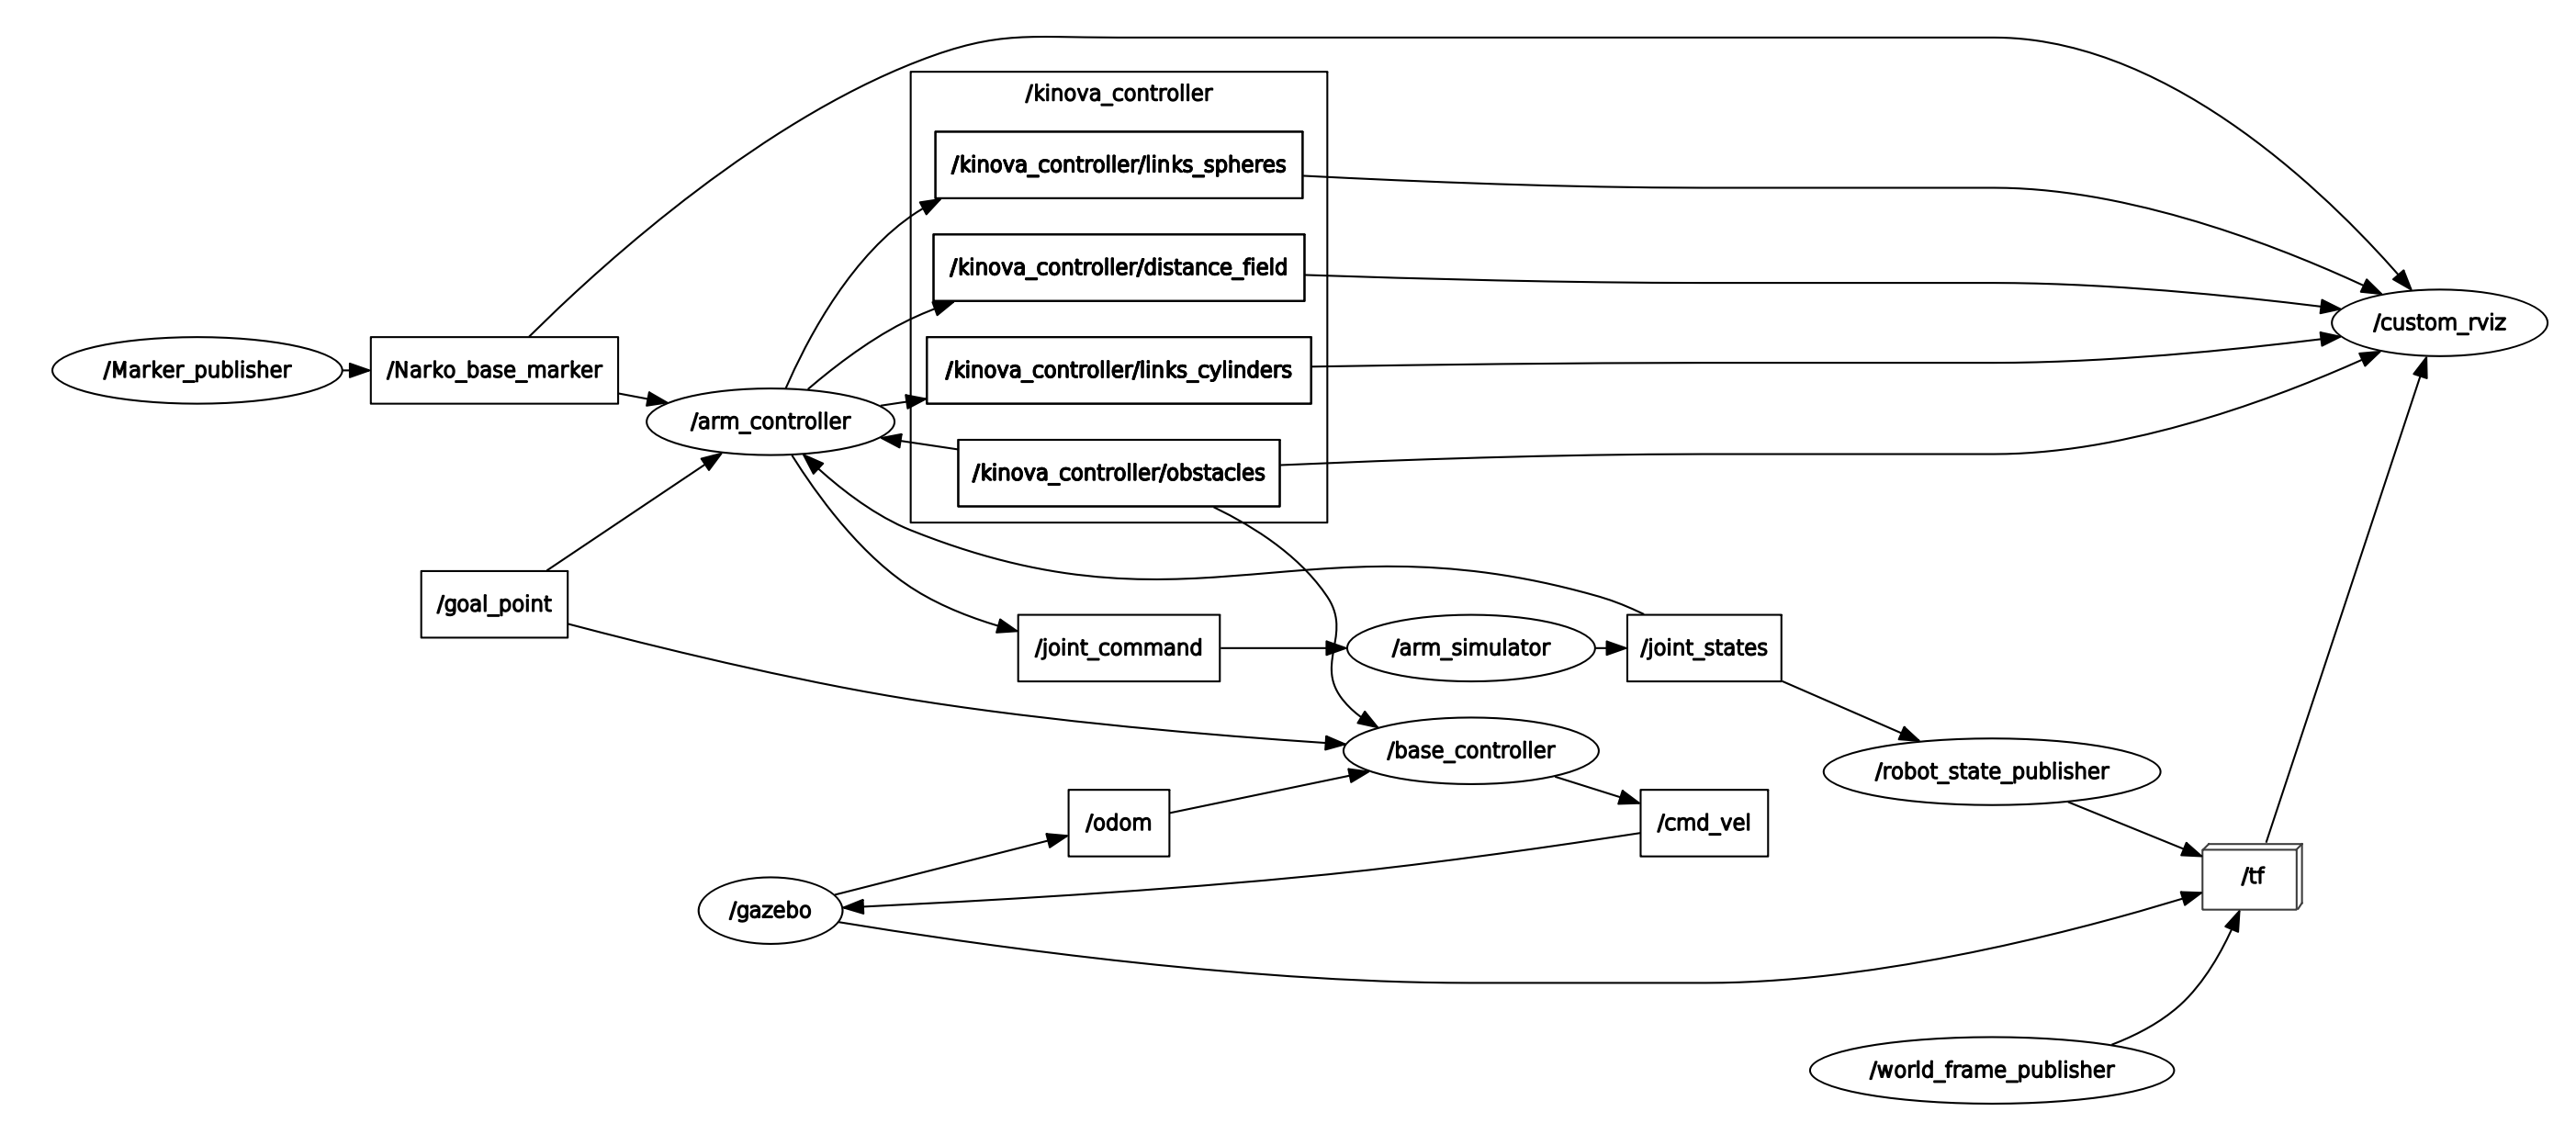
\includegraphics[width=1.0\linewidth, height=0.2\linewidth]{images/ros_graph.png}
	\caption{ROS node graph showing the communication flow between the subcomponents of the package.}
	\label{fig:rosgraph_single}
\end{figure*}

\subsection{Collision monitoring library}
This work is an extension of the the previous work. Here along with the robot arms from previous implementation, we also model the robot base such that the arms do not collide with the base while performing some actions. Along with this extension, we also implemented the base control algorithm which actively helps in monitoring and avoiding collision between the robot base and other obstacles in the workspace.

In order to monitor the distance between the links of the robot arm, obstacles, robot base in the workspace, the links are modeled as the cylinders, end effectors are modeled as spheres, and the robot base is modeled as the 3D box. This type of modeling helps in easier calculations of distance between two primitives which results in monitoring of the self collision of the arms and base. This kind of modeling helps in easier calculation of potential fields, determining the nearest points or closest points on the primitives and obstacles that helps in calculating the distances, which in turn results in real-time collision monitoring and avoidance.

\subsection{Controller} 
In this work, we follow the same architecture for the base controller as the previous work. Since we perform the collision monitoring and avoidance between the arms and the base, both the arm controller and the base controller are necessary. As per the previous work, the arm controller is controlled via a control loop which executes at a specific rate which provides the geometric locations and updates the velocity of the arms in real-time. Similarly, the base controller also controlled via a control loop which executes at a specific rate and provides information on the geometric location of the mobile base and the velocity updates. This real-time information on the positions of arm and the base helps in quicker calculation of distances and helps in collision avoidance and monitoring with self and other obstacles in the workspace.
 
\section{Implementation}
In this work, we built the extension and the base controller implementation on the ROS platform, and tested with ROS kinetic and melodic versions. There are various libraries such as Kinova Kortex library \cite{kortex}, this library provides various high and low level control APIs for handling the robotic manipulators, Kinova\_arm package that provides the design details, and implementation details for the robotic arms. Along with these libraries, in this work we make use of narko\_description for creating the robot mobile base and connect the arms and the base. The final standalone library does not depend on any ROS components, and these ROS components are used only for testing and simulation of the collision avoidance and monitoring library.

The standalone library for collision monitoring and avoidance is purely developed using the C++ programming language, we make use of ROS and python for testing, simulation, and publishing of the robot base nodes. Similar to the previous work, the package is is divided into three subcomponents, the controller for base and arms, simulator and visualization. From previous work we have the arm controller implementation based on \cite{Hoffmann}, and as an addition to this, we extended by adding the robot base as a box primitive to monitor and avoid the collision of arms with robot base. Addition to this, we implemented a base controller that helps in avoiding and monitoring the collisions with obstacles in the workspace. To visualize this, we have implemented a differential drive setup for movement and visualization of robot.

Similar to previous implementation, here we have implemented the collision avoidance part of the library in a control loop, that executes continuously to obtain the shortest distance vectors from the robot base and the obstacles. This shortest distance is then used for calculating the potential field along with the current velocity resulting in a new velocity and path for avoiding the collision and maneuvering towards goal position. This new velocity is then provided to the NarkinBase class for mapping the new velocity from Cartesian space to the robot base space.

The simulation software takes the new velocity, obstacle position and information on the potential field and generates a new position for the robot, and this new position is then passed on to the base controller such that it avoids the collision with obstacle and moves towards the goal position. This works in a loop until the robot reaches the goal position. 

A basic ROS node graph showing the communication flow between the subcomponents of the standalone package is shown in Figure \ref{fig:rosgraph_single}. Here we use the interfaces to add the obstacle to the workspace, and also to provide the goal position. For visualization, we make use of the in-built robot\_state\_publisher node and Rviz.

\section{Experiments}
ADD INFORMATION ON THE EXPERIMENTS AND TESTS PERFORMED.
\subsection{Collision Monitoring} %Brennan
The collision monitoring library has no practical measure of accuracy because of its pure mathematical basis. To assert the accuracy of the mathematics applied the distance between objects was verified using Geogebra models, and the rest of the software relies on those calculations. So the core performance measure of the collision monitoring library can be considered speed, hence the use of C++ instead of a higher level interpreted language like python. The performance test was performed on an Ubuntu 16.04 machine with a Intel Core i5-7200U 2.5GHz CPU. The following operations were timed using the C++ chrono library:
\begin{itemize}
	\item The joint initialisation of one KinovaArm and Monitor class.
	\item The combination of initialising a Sphere and adding it to the Monitor class.
	\item The updatePose function, which updates the internal kinematic representation of the arm.
	\item The distanceToObjects function, calculating the distance from each of the manipulators links to the obstacle.
	\item The distanceBetweenArmLinks function, measuring the distance from each of the links to the other links in the same manipulator.
\end{itemize}

\subsubsection{Results}
Each operation was performed 100 times with a single spherical obstacle and mean calculated to produce the final results given in Table \ref{table:Function Times} below.

\begin{table}[H]
	\centering
	\begin{tabular}{|l|l|}
		\hline
		Operation & Time (seconds) \\ \hline
		Init arm and monitor   & 0.00103831     \\ \hline
		Init and add object    & 0.00000276     \\ \hline
		Update the arm position& 0.00012871     \\ \hline
		Distance to obstacle   & 0.00026022     \\ \hline
		Distance to self links & 0.00199209     \\ \hline
	\end{tabular}
	\caption{Execution times for collision monitoring tasks}
	\label{table:Function Times}
\end{table}
From a cursory glance it is clear that the functions are quite fast, all operations take less than two milliseconds to complete, but some of the operations are not as fast as desired. From a runtime perspective the initialisation operations are not that important when is comes to overall speed, since they tend to only be run at the start of the program, and potentially at random intervals the program in the case of the obstacle initialisation. The distance to obstacles, distance between arm links, and the update function are the main operations relevant to the software refresh rate, these run every loop and depict the final update rate of the software. The update function of the arm is very fast, and the distance to obstacles function is the same only taking twice as long. It is important to note though that the time for distance to obstacles to execute relies on the number of obstacles, as the number of obstacles increases so does the time to calculate, in a linear fashion. This means that with 40 obstacles the software will be restricted to $\sim$ 10Hz. Assuming only one obstacle the other large impact to overall performance in the distance to self links operation, taking up over four times the time used by the other two core functions combined. This was somewhat expected, if not to this extent, since the software was designed for portability in mind, which limits the possible optimisations available, still further investigation into the limiting factors should be performed. The final core loop time for the collision monitoring library is a little over 4.7 milliseconds, which would give a update rate of $\sim$ 250hz, but this would gain significant benefits from the exclusion of the distance to own links monitoring functions.



\subsection{Single arm obstacle avoidance} %Sam
% In order to visualize the obstacle avoidance we first simulated a single instance of the Kinova\textsuperscript{\tiny\textregistered} Gen3 robotic manipulator and placed obstacles in its workspace, as seen in Fig. \ref{fig:one_arm}. We then provided different commands to find tune the relevant parameters and assess the effectiveness of the algorithm. 
 To assess the effectiveness of the algorithm we place several obstacles in the vicinity of the manipulator, and then command it to move between points in the workspace. First, we used the same set of obstacles, initial point and goal point for two experiments with two different values for $\gamma$ as seen in Figure 4. When $\gamma=0$ there is no influence of the potential field in the velocity, hence the end effector does not avoid the obstacle. Whereas when $\gamma=35$ the effect of the potential field steers the end effector away from the obstacle in its path. From these results we can assess that the DMP will converge to the goal point, and the value of $\gamma$ has an impact in the effectiveness of the algorithm. 

\begin{figure}[H]
	\centering
	\label{potential}
	\begin{subfigure}[t]{0.20\textwidth}
		\centering
		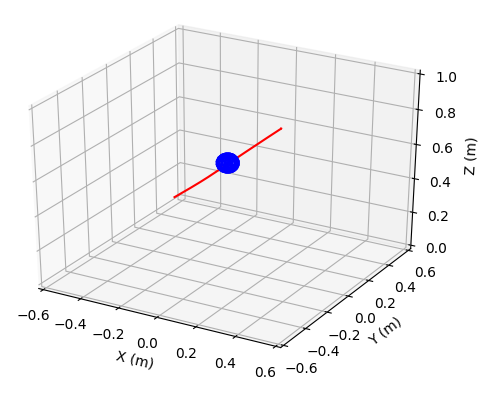
\includegraphics[scale=0.35]{images/no_potential.png}
		\caption{$\gamma = 0$}
	\end{subfigure}%
	~ 
	\begin{subfigure}[t]{0.20\textwidth}
		\centering
		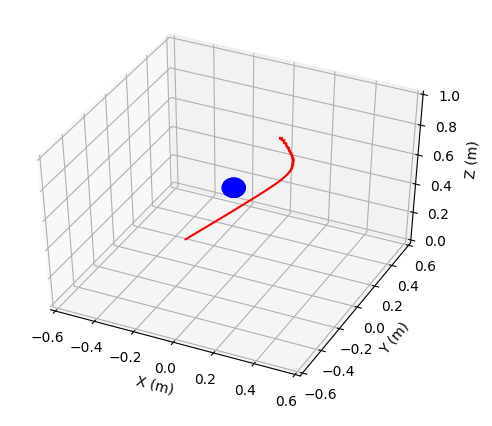
\includegraphics[scale=0.35]{images/yes_potential.png}
		\caption{$\gamma = 35$}
	\end{subfigure}
	\caption{Movement with different values for $\gamma$}
\end{figure}

In Figure \ref{fig:potential_field} we can observe the behaviour of the potential field when several obstacles are nearby. Note that the potential field's magnitude is larger when the end effector is approaching the obstacles and gets smaller after it passes the obstacles. This is the effect of the steering angle, as when the end effector passes the obstacles the angle between the current velocity and the obstacles is large. It should also be noted that the direction of the potential field effect is not uniform between small steps.

\begin{figure}[H]
	\centering
	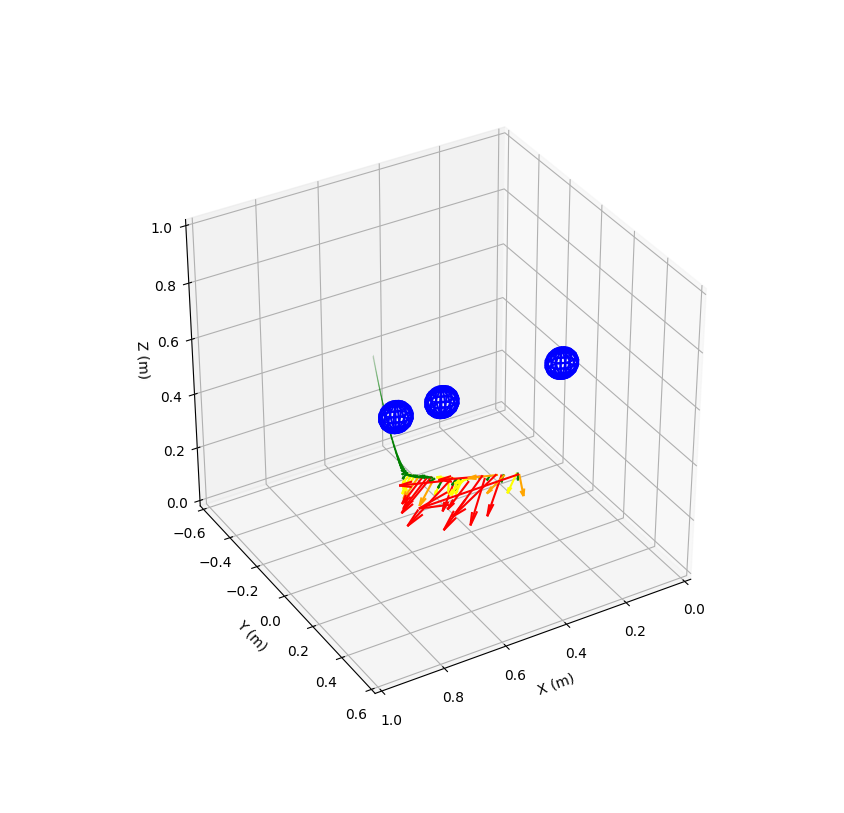
\includegraphics[scale=0.30]{images/potential_field.png}
	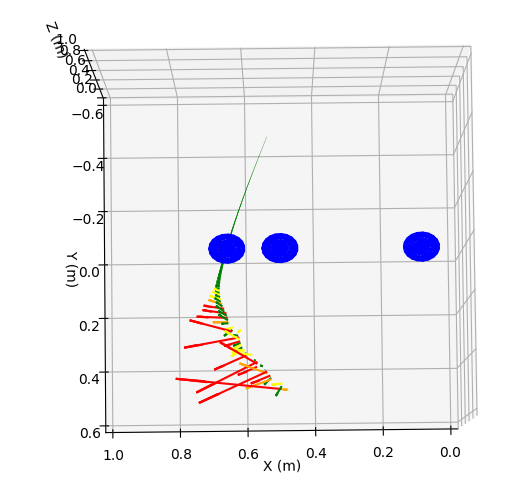
\includegraphics[scale=0.30]{images/potential_field_top.png}
	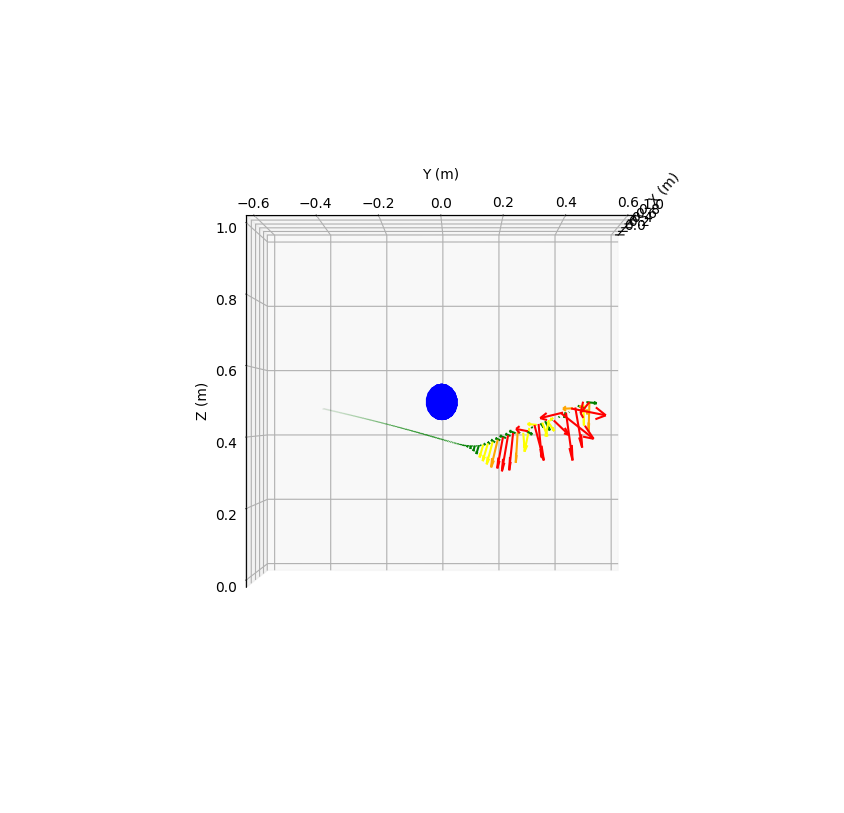
\includegraphics[scale=0.30]{images/potential_field_side.png}
	\caption{Potential field generated during the movement}
	\label{fig:potential_field}
\end{figure}

For one of the experiments we placed several obstacles in the workspace and command it to move between points. The results of the collision avoidance algorithm can be seen from several perspectives in fig \ref{fig:one_arm_avoidance}. The red line is the path of the end effector from the initial point to the goal. In fig \ref{fig:one_arm_avoidance_vector} the velocity vectors in their respective point in time can be observed. 

\begin{figure}[H]
	\centering
	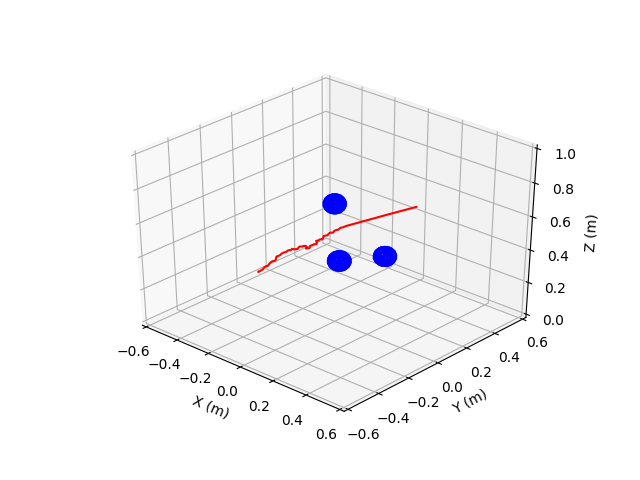
\includegraphics[scale=0.30]{images/one_arm_three_obstacles.png}
	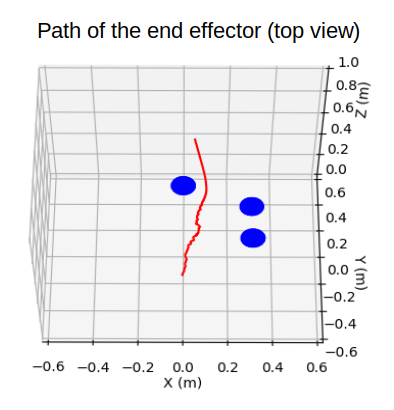
\includegraphics[scale=0.30]{images/one_arm_three_obstacles_top.png}
	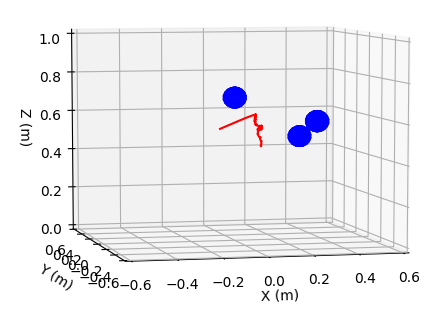
\includegraphics[scale=0.30]{images/one_arm_three_obstacles_side.png}
	\caption{Path of the end effector as it moves through obstacles}
	\label{fig:one_arm_avoidance}
\end{figure}

\begin{figure}[H]
	\centering
	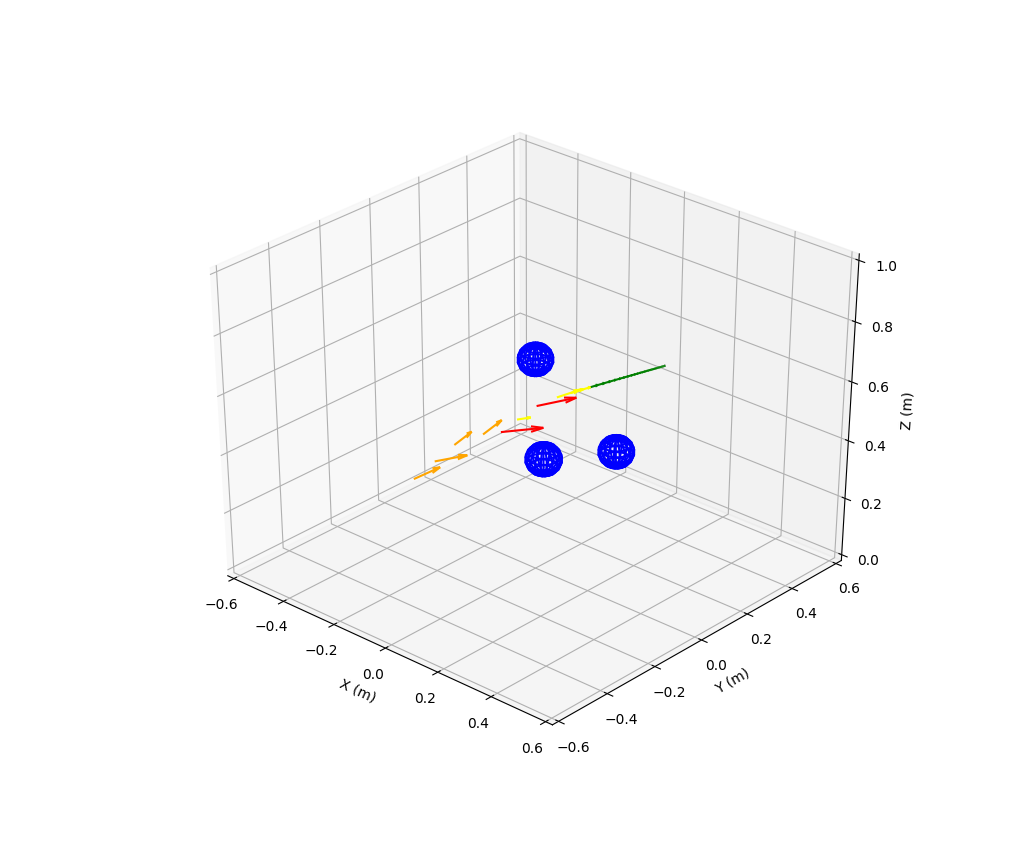
\includegraphics[scale=0.30]{images/one_arm_three_obstacles_vector.png}
	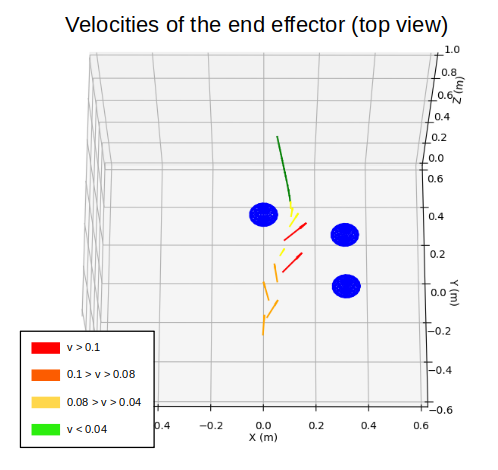
\includegraphics[scale=0.30]{images/one_arm_three_obstacles_top_vector.png}
	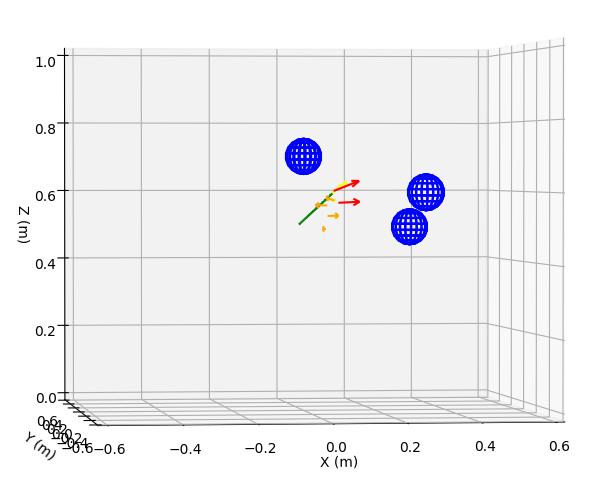
\includegraphics[scale=0.30]{images/one_arm_three_obstacles_side_vector.png}
	\caption{Cartesian velocities generated by the algorithm}
	\label{fig:one_arm_avoidance_vector}
\end{figure}

As it can be observed from Figure \ref{fig:one_arm_avoidance} and Figure \ref{fig:one_arm_avoidance_vector} the collision avoidance algorithm can generate velocities that avoid several obstacles without problems. 

\subsection{Dual arm collision avoidance} %Sam

In order for two manipulators to operate with intersecting workspaces it is important that they do not collide with each other. In this experiment we simulated two instances of the Kinova arm placed close to each other so their workspaces would overlap. Each arm is individually controlled, meaning we could place one arm on the path of the other to assess if the arms avoided collisions. An example setup can be seen in Figure \ref{fig:two_arms}. The objective is to assess if the arms avoid colliding with each other during operation.

\begin{figure}[H]
	\centering
	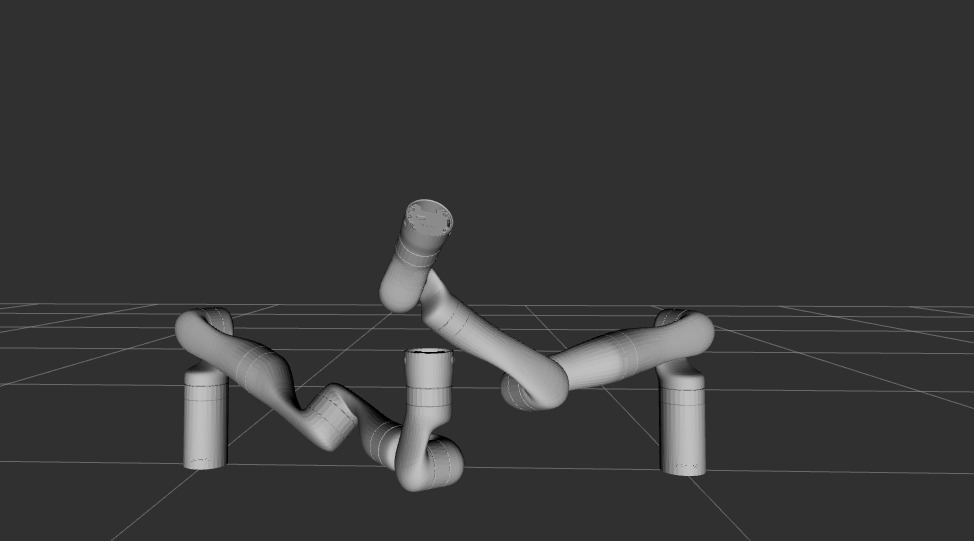
\includegraphics[scale=0.15]{images/two_arms.jpeg}
	\caption{Two arms sharing a space}
	\label{fig:two_arms}
\end{figure}

In Figure \ref{fig:two_arm_avoidance} the path of the end effector of first Kinova arm can be seen as well as the pose of the second arm. The pose of the second arm remained constant during the movement of the first arm. 

\begin{figure}[H]
	\centering
	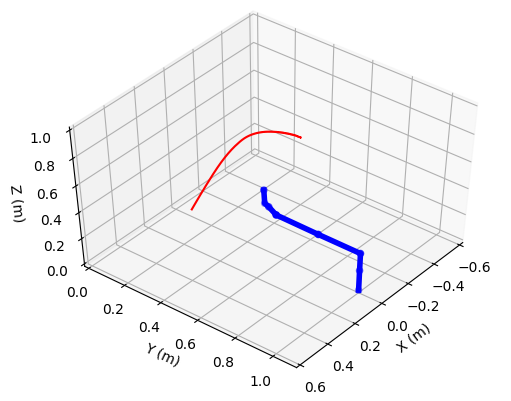
\includegraphics[scale=0.25]{images/two_arms.png}
	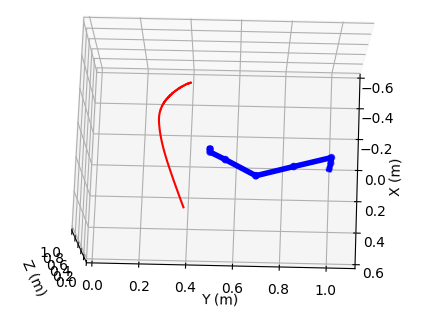
\includegraphics[scale=0.25]{images/two_arms_top.png}
	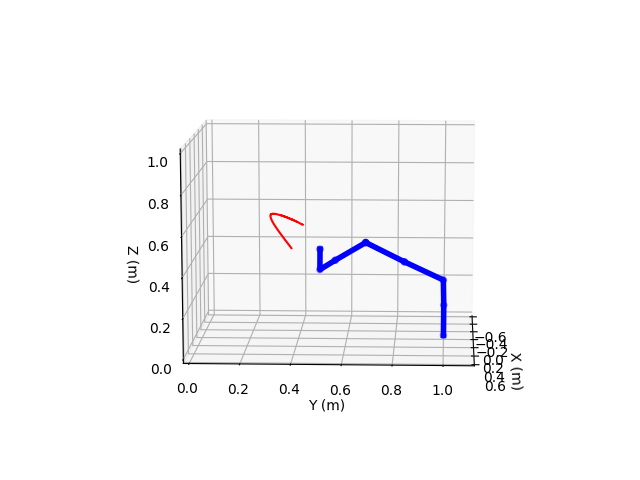
\includegraphics[scale=0.25]{images/two_arms_side.png}
	\caption{Path of the end effector of one arm}
	\label{fig:two_arm_avoidance}
\end{figure}

\begin{figure}[H]
	\centering
	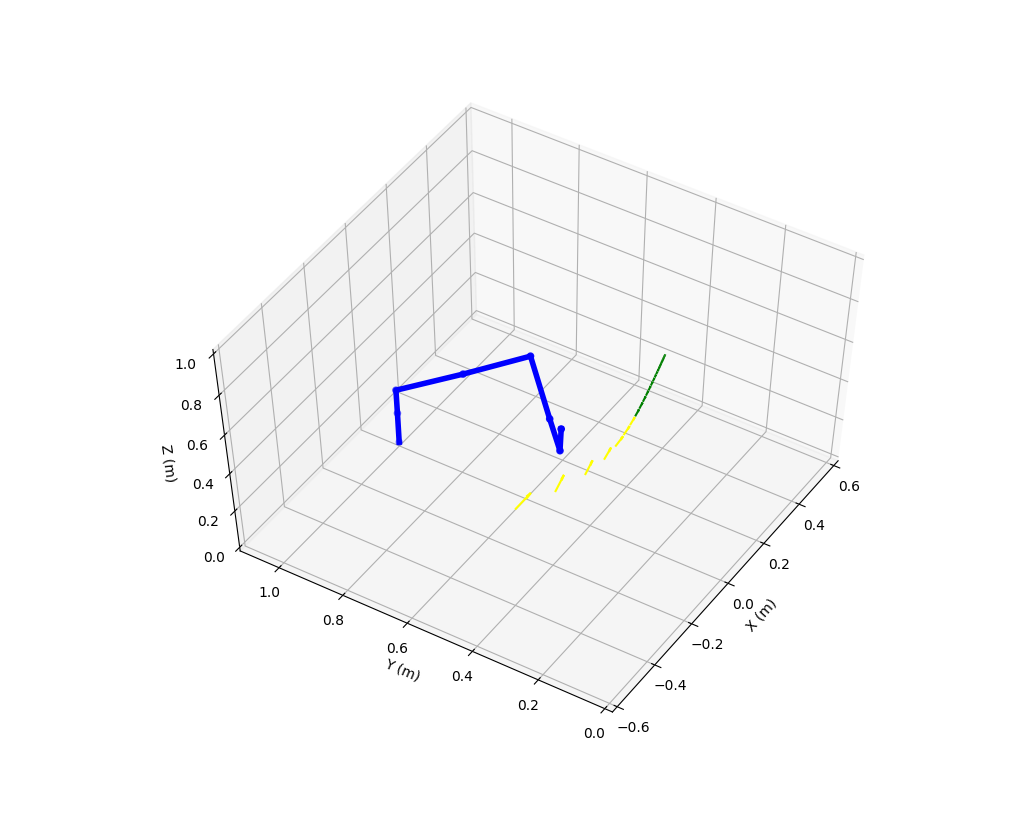
\includegraphics[scale=0.25]{images/two_arms_vector.png}
	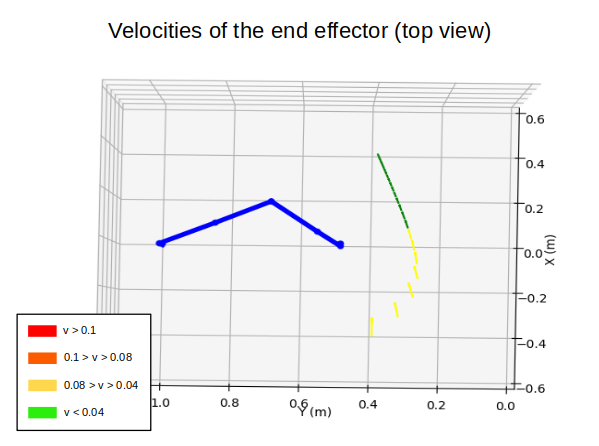
\includegraphics[scale=0.25]{images/two_arms_vector_top.png}
	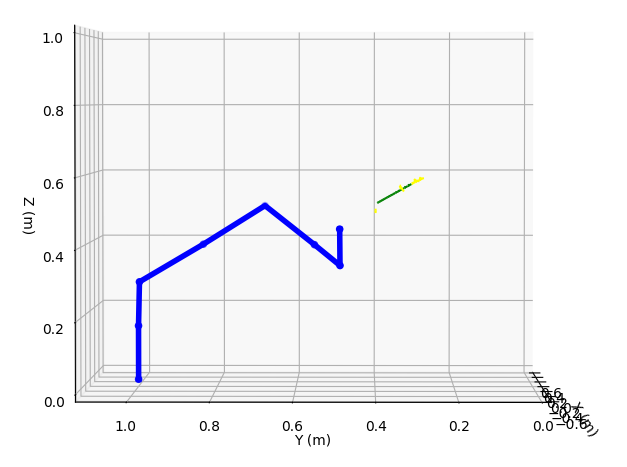
\includegraphics[scale=0.25]{images/two_arms_vector_side.png}
	\caption{Cartesian velocities generated}
	\label{fig:two_arm_avoidance_vector}
\end{figure}

From these results we can see that a long as the geometric representation of the two arms is accurate, the collision avoidance algorithm can be use to avoid collisions between the arms. The collision avoidance algorithm only monitors the end effector of the moving robot, this means that not all collision between the two arms can be avoided. To fix this a null space control algorithm would need to be implemented. 

\section{Use cases}

\subsection{Arm}
Since this work is an extension of previous work, all the features that were implemented related to the arms still functions and can be used to create and experiment with multiple number of arms. Considering single arm, the arm controller looks and helps in avoiding and monitoring the collision of end-effector with the obstacles in the workspace. Considering dual arms, the links and joints of the arms are represented as obstacles, hence both arms do not collide with each other and also they do not collide with the obstacles. Any number of obstacles can be added to the workspace using the interfacer provided in the library. Similarly, the library is capable of handling more than two arms and they have to be configured before execution of the library.

\subsection{Base}
In this work, the robot base is modeled as a 3D box or can be referred to as a cuboid. This cuboid is treated as an obstacle from the arm controller point of view and this helps in avoiding and monitoring of self collision between arm and the base. This cuboid representation acts as a generic representation since most of the robot's base is either of a cuboid shape or of cylindrical shape and can be enclosed using a cuboid. Along with this, the base controller implementation looks out for obstacles in the workspace and actively monitors and avoids collision.

\section{Conclusion}
For robotic manipulators to be used in a human environment they first need to have the ability to adapt in constantly changing, dynamic environments. This can be done in a robust and safe manner using a combination of two different methods discussed by H. Hoffmann et al. \cite{Hoffmann} and O. Khatib \cite{Khatib}. By implementing the obstacle monitoring by O. Khatib \cite{Khatib} and the collision avoidance by H. Hoffmann et al. \cite{Hoffmann}, along with monitoring collisions for all links, robotic manipulators are more resilient to changes in obstacle and goal placement. The final collision monitoring library can have an update rate of $\sim$ 200Hz with all features enabled, this is a viable update rate, but this would become drastically impacted if more that 10 obstacles were to be added to the environment. % Sam can sumarise about his results.
From the experiments it can be concluded that the DMPs used in this algorithm converge to the goal, and that the potential field term influences the end effector's path to steer away from obstacles. 
It can also be observed that the effectiveness of the algorithm is dependent on the parameters of the DMP equation, hence it is important for a developer to fine tune this parameters until a certain level of performance is reached.
 
While the algorithm produced gives some significant benefits over previous methods, there is still a lot of potential improvements. The collision monitoring library could benefit greatly from some optimisation of the self collision functions, along with the addition of more shapes. The current shapes are a basic sphere and capsule, with the addition of an n-ellipsoid primitive a large majority of basic shapes and structures could be constructed by the combination of the primitives. % Sam can add any future works given from his section or results.
Finally, in order to avoid more serious collisions, the algorithm should consider the entire body of the manipulator rather than just the end effector. 

%The computation of the distances between different kinds of objects is not easy, one needs to take into consideration different scenarios, otherwise, the main algorithm might fail. Further work on this area could be adding other kinds of shapes.


\addtolength{\textheight}{-12cm}   % This command serves to balance the column lengths
                                  % on the last page of the document manually. It shortens
                                  % the textheight of the last page by a suitable amount.
                                  % This command does not take effect until the next page
                                  % so it should come on the page before the last. Make
                                  % sure that you do not shorten the textheight too much.

%%%%%%%%%%%%%%%%%%%%%%%%%%%%%%%%%%%%%%%%%%%%%%%%%%%%%%%%%%%%%%%%%%%%%%%%%%%%%%%%



%%%%%%%%%%%%%%%%%%%%%%%%%%%%%%%%%%%%%%%%%%%%%%%%%%%%%%%%%%%%%%%%%%%%%%%%%%%%%%%%
\section*{Appendix}
The code for the collision monitoring library is accessible at the following link: \url{https://github.com/Sreeni1204/sdp\_ws20\_collision\_monitoring\_for\_mobile\_manipulators}

%%%%%%%%%%%%%%%%%%%%%%%%%%%%%%%%%%%%%%%%%%%%%%%%%%%%%%%%%%%%%%%%%%%%%%%%%%%%%%%%
\section*{Acknowledgements}
We would like to thank Djordje Vukcevic for his support and motivation throughout the course of this project.

%%%%%%%%%%%%%%%%%%%%%%%%%%%%%%%%%%%%%%%%%%%%%%%%%%%%%%%%%%%%%%%%%%%%%%%%%%%%%%%%


\begin{thebibliography}{10}
	
\bibitem{Khatib} O. Khatib, “Real-Time Obstacle Avoidance for Manipulators and Mobile Robots” The International Journal of Robotics Research, vol. 5, no. 1, pp. 90–98, Mar. 1986, doi: 10.1177/027836498600500106.
\bibitem{Hoffmann} H. Hoffmann, P. Pastor, D.-H. Park, and S. Schaal, “Biologically-inspired dynamical systems for movement generation: Automatic real-time goal adaptation and obstacle avoidance,” in 2009 IEEE International Conference on Robotics and Automation, Kobe, May 2009, pp. 2587–2592, doi: 10.1109/ROBOT.2009.5152423.
\bibitem{Fadalil} M. S. Fadali and A. Visioli, “Introduction to Digital Control,” in Digital Control Engineering, Elsevier, 2013, pp. 1–8.
\bibitem{Adee} S. Adee, “Dean Kamen’s ‘Luke Arm’ Prosthesis Readies for Clinical Trials - IEEE Spectrum,” IEEE Spectrum: Technology, Engineering, and Science News, Feb. 01, 2008. https://spectrum.ieee.org/biomedical/bionics/dean-kamens-luke-arm-prosthesis-readies-for-clinical-trials (accessed Jun. 25, 2020).
\bibitem{Janabi-Sharif} F. Janabi-Sharifi and D. Vinke, “Integration of the artificial potential field approach with simulated annealing for robot path planning,” in Proceedings of 8th IEEE International Symposium on Intelligent Control, Aug. 1993, pp. 536–541, doi: 10.1109/ISIC.1993.397640.
\bibitem{rodrigues}  Belongie, Serge. "Rodrigues' Rotation Formula." From MathWorld--A Wolfram Web Resource, created by Eric W. Weisstein. https://mathworld.wolfram.com/RodriguesRotationFormula.html 
\bibitem{kortex} Kinovarobotics/ros\_kortex. Kinova Robotics, 2020.
\bibitem{GJK} E. G. Gilbert, D. W. Johnson and S. S. Keerthi, "A fast procedure for computing the distance between complex objects in three-dimensional space," in IEEE Journal on Robotics and Automation, vol. 4, no. 2, pp. 193-203, April 1988, doi: 10.1109/56.2083.
\bibitem{3ddet} AABB · 3DCollisions - \url{https://gdbooks.gitbooks.io/3dcollisions/content/Chapter1/aabb.html}, Accessed on 03/07/2021
%\bibitem{Velliste} M. Velliste, S. Perel, M. C. Spalding, A. S. Whitford, and A. B. Schwartz, “Cortical control of a prosthetic arm for self-feeding,” Nature, vol. 453, no. 7198, Art. no. 7198, Jun. 2008, doi: 10.1038/nature06996.



\end{thebibliography}


\end{document}